\documentclass[12pt]{report}

\usepackage[a4paper, left=2.5cm, right=2.5cm, top=3cm, bottom=3cm]{geometry}
\usepackage{graphicx}
\usepackage{glossaries}
\usepackage{titling}
\usepackage{pdfpages}
\usepackage{listings}
\lstset{language=SQL}
\usepackage{hyperref}
\usepackage{appendix}
\usepackage{tikz}
\usepackage{caption}
\usepackage{float}



\renewcommand{\appendixpagename}{Annexes}
\renewcommand{\appendixtocname}{Annexes}

\setlength{\parindent}{0pt}

\title{Winventory \\ \large BDR-Projet}
\author{Lestiboudois Maxime \& \\Parisod Nathan \& \\Surbeck Léon}
\date{24.01.2025}

% Redéfinir \maketitle pour inclure l'image sous le titre
\pretitle{\begin{center}\Huge\bfseries}
\posttitle{\par\end{center}\vspace{0.5cm}
\begin{center}
\hspace*{2cm}
\includegraphics[scale = 1]{images/Logo_court}
\end{center}\vspace{0.5cm}}


% Document
\begin{document}
    \maketitle
    \tableofcontents
    \newpage

%%%%%%%%%%%%%%%%%%%%
%%  Introduction  %%
%%%%%%%%%%%%%%%%%%%%
    \section*{Introduction}
    \addcontentsline{toc}{section}{Introduction}

    Le projet \textbf{Winventory} a pour ambition de concevoir une base de données relationnelle performante et innovante,
    spécialement pensée pour gérer les inventaires de vins, bières, spiritueux, boissons non alcoolisées, apéritifs et équipements.
    \newline
    Grâce à une solution centralisée, Winventory simplifiera la gestion des stocks, le suivi des acquisitions et les
    retraits de produits, tout en offrant des fonctionnalités avancées d’analyse et de reporting via une interface utilisateur intuitive.
    \newline
    \newline
    Le système offrira une gestion centralisée des inventaires sur plusieurs magasins, rendant possible le transfert de
    stock entre différents sites tout en permettant une supervision globale. Par ailleurs, l’intégration des historiques
    d’achat des clients permettra de mieux anticiper les besoins, d’optimiser la préparation des stocks et de soutenir
    les actions marketing à travers des offres personnalisées et des prédictions sur les comportements d'achat.
    Enfin, Wineventory s’appuiera sur la robustesse de PostgreSQL pour garantir une performance optimale dans le traitement
    des requêtes complexes et la production de rapports détaillés.
    \newline Toutes les requêtes SQL seront écrites manuellement afin de garantir un contrôle total et d’assurer une transparence complète du système.


%%%%%%%%%%%%%%%%%%%%
%%    Modèle EA   %%
%%%%%%%%%%%%%%%%%%%%
    \section*{Modèle EA}
    \addcontentsline{toc}{section}{Modèle EA}

    \begin{center}
        \includegraphics[scale = 0.6]{images/Schema_UML}
    \end{center}\vspace{0.5cm}

%%%%%%%%%%%%%%%%%%%%
%% Modèle relationnel %%
%%%%%%%%%%%%%%%%%%%%
    \section*{Modèle relationnel}
    \addcontentsline{toc}{section}{Modèle relationnel}

    \begin{itemize}
        \item \textbf{Provenance}
        \begin{itemize}
            \item \underline{id}, pays, région, producteur
        \end{itemize}

        \item \textbf{Produit}
        \begin{itemize}
            \item \underline{idProduit}, idProvenance, nom, tauxAlcool
            \item \textit{idProvenance} référence \textit{Provenance.id}, \textit{idProvenance NOT NULL}
        \end{itemize}

        \item \textbf{Article}
        \begin{itemize}
            \item \underline{idProduit, volume, recipient}, prix, datePeremption, dateFinDeVente
            \item \textit{idProduit} référence \textit{Produit.id}
        \end{itemize}

        \item \textbf{MouvementStock}
        \begin{itemize}
            \item \underline{id}, idMagasin, idProduit, volume, recipient, date, quantite
            \item \textit{idMagasin} référence \textit{Magasin.id}
            \item \textit{idProduit, volume, recipient} référence \textit{Article.idProduit, volume, recipient}
            \item \textit{idProduit, volume, recipient NOT NULL}
        \end{itemize}

        \item \textbf{Magasin}
        \begin{itemize}
            \item \underline{id}, nom, adresse, dateFermeture
        \end{itemize}

        \item \textbf{Vendeur}
        \begin{itemize}
            \item \underline{id}, idMagasin, nom, salaire, estActif
            \item \textit{idMagasin} référence \textit{Magasin.id}, \textit{idMagasin NOT NULL}
        \end{itemize}

        \item \textbf{Vente}
        \begin{itemize}
            \item \underline{idMouvementStock}, idVendeur, idClient
            \item \textit{idMouvementStock} référence \textit{MouvementStock.id}
            \item \textit{idVendeur} référence \textit{Vendeur.id}, \textit{idVendeur NOT NULL}
            \item \textit{idClient} référence \textit{Client.id}, \textit{idClient NOT NULL}
        \end{itemize}

        \item \textbf{Approvisionnement}
        \begin{itemize}
            \item \underline{idMouvementStock}, dateCommande
            \item \textit{idMouvementStock} référence \textit{MouvementStock.id}
        \end{itemize}

        \item \textbf{Client}
        \begin{itemize}
            \item \underline{id}, nom, adresse, email, pointDeFidelite, annéeNaissance
            \item \textit{email UNIQUE}
        \end{itemize}

        \item \textbf{Fournisseur}
        \begin{itemize}
            \item \underline{id}, nom, adresse, numeroTelephone
        \end{itemize}

        \item \textbf{Approvisionnement\_Fournisseur}
        \begin{itemize}
            \item \underline{idMouvementStock, idFournisseur}
            \item \textit{idMouvementStock} référence \textit{MouvementStock.id}
            \item \textit{idFournisseur} référence \textit{Fournisseur.id}
        \end{itemize}

    \end{itemize}

%%%%%%%%%%%%%%%%%%%%
%Création de tables%
%%%%%%%%%%%%%%%%%%%%
    \section*{Création de tables}
    \addcontentsline{toc}{section}{Création de tables}

    Voici le script SQL nous permettant de créer les tables de notre base de données:
    \newline
    \newline
    \begin{lstlisting}[breaklines=true]
        CREATE TABLE IF NOT EXISTS Provenance(
    id SERIAL,
    pays VARCHAR(80),
    region VARCHAR(80),
    producteur VARCHAR(80),
    CONSTRAINT PK_Provenance PRIMARY KEY (id)
);

--CREATE TYPE typeRecipient AS ENUM ('bouteille', 'canette');

CREATE TABLE IF NOT EXISTS Produit(
  idProduit SERIAL,
  idProvenance INTEGER NOT NULL,
    nom VARCHAR(80) NOT NULL,
    tauxAlcool DOUBLE PRECISION NOT NULL,
    CONSTRAINT PK_Produit PRIMARY KEY (idProduit),
    constraint FK_idProvenance foreign KEY(idProvenance) references Provenance(id) ON UPDATE CASCADE ON DELETE RESTRICT
);

CREATE TABLE IF NOT EXISTS Article(
    idProduit INTEGER,
    volume INTEGER,
    recipient typeRecipient,
    prix DOUBLE PRECISION NOT NULL,
    datePeremption DATE NOT NULL,
    dateFinDeVente DATE,
    CONSTRAINT PK_Article PRIMARY KEY (idProduit, volume, recipient),
    CONSTRAINT FK_Article_Produit FOREIGN KEY (idProduit) REFERENCES Produit(idProduit) ON UPDATE CASCADE ON DELETE RESTRICT
);

CREATE TABLE IF NOT EXISTS Magasin(
    id SERIAL,
    nom VARCHAR(80) NOT NULL,
    adresse VARCHAR(350) NOT NULL,
    dateFermeture DATE,
    CONSTRAINT PK_Magasin PRIMARY KEY (id)
);

CREATE TABLE IF NOT EXISTS MouvementStock(
    id SERIAL,
    idMagasin INTEGER NOT NULL,
    idProduit INTEGER NOT NULL,
    volume INTEGER NOT NULL,
    recipient typeRecipient NOT NULL,
    date DATE,
    quantite INTEGER,
    CONSTRAINT PK_MouvementStock PRIMARY KEY (id),
    CONSTRAINT FK_MouvementStock_Magasin FOREIGN KEY (idMagasin) REFERENCES Magasin(id) ON UPDATE CASCADE ON DELETE CASCADE,
    CONSTRAINT FK_MouvementStock_Article FOREIGN KEY (idProduit, volume, recipient) REFERENCES Article(idProduit, volume, recipient) ON UPDATE CASCADE ON DELETE CASCADE
);

CREATE TABLE IF NOT EXISTS Vendeur(
    id SERIAL,
    idMagasin INTEGER NOT NULL,
    nom VARCHAR(80),
    salaire DOUBLE PRECISION,
    estActif BOOL NOT NULL,
    CONSTRAINT PK_Vendeur PRIMARY KEY (id),
    CONSTRAINT FK_Vendeur_Magasin FOREIGN KEY (idMagasin) REFERENCES Magasin(id) ON UPDATE CASCADE ON DELETE CASCADE
);

CREATE TABLE IF NOT EXISTS Client(
    id SERIAL,
    nom VARCHAR(80),
    adresse VARCHAR(150),
    email VARCHAR(100) UNIQUE,
    pointDeFidelite INTEGER,
    anneeNaissance INTEGER,
    CONSTRAINT PK_Client PRIMARY KEY (id)
);

CREATE TABLE IF NOT EXISTS Vente(
    idMouvementStock INTEGER,
    idVendeur INTEGER NOT NULL,
    idClient INTEGER NOT NULL,
    CONSTRAINT PK_Vente PRIMARY KEY (idMouvementStock),
    CONSTRAINT FK_Vente_MouvementStock FOREIGN KEY (idMouvementStock) REFERENCES MouvementStock(id) ON UPDATE CASCADE ON DELETE CASCADE,
    CONSTRAINT FK_Vente_Vendeur FOREIGN KEY (idVendeur) REFERENCES Vendeur(id) ON UPDATE CASCADE ON DELETE RESTRICT,
    CONSTRAINT FK_Vente_Client FOREIGN KEY (idClient) REFERENCES Client(id) ON UPDATE CASCADE ON DELETE RESTRICT
);

CREATE TABLE IF NOT EXISTS Approvisionnement(
    idMouvementStock INTEGER,
    dateCommande DATE NOT NULL,
    CONSTRAINT PK_Approvisionnement PRIMARY KEY (idMouvementStock),
    CONSTRAINT FK_Approvisionnement_Approvisionnement FOREIGN KEY (idMouvementStock) REFERENCES MouvementStock(id) ON UPDATE CASCADE ON DELETE cascade,
    CONSTRAINT check_DateCommande CHECK (dateCommande <= CURRENT_DATE)
);

CREATE TABLE IF NOT EXISTS Fournisseur(
    id SERIAL,
    nom VARCHAR(80),
    adresse VARCHAR(150),
    numeroTelephone VARCHAR(30),
    CONSTRAINT PK_Fournisseur PRIMARY KEY (id)
);

CREATE TABLE IF NOT EXISTS Approvisionnement_Fournisseur(
    idMouvementStock INTEGER,
    idFournisseur INTEGER,
    CONSTRAINT PK_Approvisionnement_Fournisseur PRIMARY KEY (idMouvementStock, idFournisseur),
    CONSTRAINT FK_Approvisionnement_Fournisseur_idMouvementStock FOREIGN KEY (idMouvementStock) REFERENCES Approvisionnement(idMouvementStock) ON UPDATE CASCADE ON DELETE CASCADE,
    CONSTRAINT FK_Approvisionnement_Fournisseur_idFournisseur FOREIGN KEY (idFournisseur) REFERENCES Fournisseur(id) ON UPDATE CASCADE ON DELETE CASCADE
);
    \end{lstlisting}

%%%%%%%%%%%%%%%%%%%%
%REmplissage de tables%
%%%%%%%%%%%%%%%%%%%%
    \section*{Remplissage des tables}
    \addcontentsline{toc}{section}{Remplissage des tables}

    Ce script SQL suivant nous a permis de remplir les tables de notre base de données:
    \newline
    \newline
    \begin{lstlisting}[breaklines=true]
        -- Remplissage de la table Provenance
INSERT INTO Provenance (pays, region, producteur) VALUES
('France', 'Bordeaux', 'Château Margaux'),
('Italie', 'Toscane', 'Antinori'),
('Espagne', 'Ribera del Duero', 'Bodega Vega Sicilia'),
('USA', 'Napa Valley', 'Robert Mondavi'),
('France', 'Champagne', 'Moët & Chandon');

-- Remplissage de la table Produit
INSERT INTO Produit (nom, tauxAlcool, idProvenance) VALUES
('Vin Rouge Bordeaux', 13.5, 1),
('Vin Blanc Chardonnay', 12.0, 2),
('Champagne Brut', 12.5, 2),
('Whisky Single Malt', 40.0, 3),
('Bière Blonde', 5.0, 1);

-- Remplissage de la table Article
INSERT INTO Article (idProduit, volume, recipient, prix, datePeremption, dateFinDeVente) VALUES
(1, 750, 'bouteille', 45.99, '2025-12-31', NULL),
(1, 1500, 'bouteille', 89.99, '2025-12-31', NULL),
(2, 750, 'bouteille', 35.99, '2024-11-30', '2024-10-01'),
(3, 750, 'bouteille', 55.00, '2026-06-30', NULL),
(4, 700, 'bouteille', 120.00, '2030-01-01', NULL),
(5, 330, 'canette', 2.50, '2023-12-31', '2023-11-01');

-- Remplissage de la table Magasin
INSERT INTO Magasin (nom, adresse, dateFermeture) VALUES
('Cave de Paris', '12 rue de la Paix, Paris, France', NULL),
('Wine World', '45 High Street, London, UK', NULL),
('Enoteca Roma', 'Via Condotti, 25, Rome, Italy', '2025-01-01');

-- Remplissage de la table MouvementStock
INSERT INTO MouvementStock (idMagasin, idProduit, volume, recipient, date, quantite) VALUES
(1, 1, 750, 'bouteille', '2024-01-10', 100),
(1, 2, 750, 'bouteille', '2024-01-15', 50),
(2, 3, 750, 'bouteille', '2024-01-20', 30),
(2, 5, 330, 'canette', '2023-12-01', 500),
(3, 4, 700, 'bouteille', '2023-11-25', 20);

-- Remplissage de la table Vendeur
INSERT INTO Vendeur (idMagasin, nom, salaire, estActif) VALUES
(1, 'Alice Dupont', 2500.00, TRUE),
(2, 'John Smith', 2200.00, TRUE),
(3, 'Giulia Rossi', 2400.00, FALSE);

-- Remplissage de la table Client
INSERT INTO Client (nom, adresse, email, pointDeFidelite, anneeNaissance) VALUES
('Paul Morel', '34 avenue des Champs, Paris, France', 'paul.morel@example.com', 120, 1985),
('Anna Garcia', '23 Carrer Major, Barcelona, Spain', 'anna.garcia@example.com', 80, 1990),
('James Taylor', '56 Broadway, New York, USA', 'james.taylor@example.com', 200, 1980);

-- Remplissage de la table Vente
INSERT INTO Vente (idMouvementStock, idVendeur, idClient) VALUES
(1, 1, 1),
(2, 1, 2),
(3, 2, 3);

-- Remplissage de la table Approvisionnement
INSERT INTO Approvisionnement (idMouvementStock, dateCommande) VALUES
(4, '2023-11-01'),
(5, '2023-10-15');

-- Remplissage de la table Fournisseur
INSERT INTO Fournisseur (nom, adresse, numeroTelephone) VALUES
('Distrib Vins France', '45 rue du Vin, Bordeaux, France', '+33 5 56 00 00 01'),
('Champagne Select', '12 avenue de la Champagne, Reims, France', '+33 3 26 00 00 02'),
('Global Spirits', '99 Whiskey Lane, Dublin, Ireland', '+353 1 00 00 03');

-- Remplissage de la table Approvisionnement_Fournisseur
INSERT INTO Approvisionnement_Fournisseur (idMouvementStock, idFournisseur) VALUES
(4, 1),
(5, 3);
    \end{lstlisting}


%%%%%%%%%%%%%%%%%%%%
%Description de l'apps%
%%%%%%%%%%%%%%%%%%%%
    \section*{Description de l'application}
    \addcontentsline{toc}{section}{Description de l'application}
    L'application permet de gérer et de voir le contenu des stocks d'un magasin (pour l'instant).
    \newline
    \subsection*{Accès à l'application}
    \addcontentsline{toc}{subsection}{Accès à l'application}
    Pour accéder à l'application, il y a deux manières possibles:
    \begin{enumerate}
        \item en local, il suffit de cloner le répertoire Github au lieu suivant : \href{https://github.com/La-Kirby-Team/BDR-Project}{https://github.com/La-Kirby-Team/BDR-Project}.
        \newline Une fois le répertoire cloné en local, il suffit de suivre les instructions contenues dans le fichier \href{https://github.com/La-Kirby-Team/BDR-Project/blob/main/README.md}{README.md} (voir Annexe 1)
        \item l'application est également disponible sur le site \href{winventory.duckdns.org}{winventory.duckdns.org}.
    \end{enumerate}

    Tout le monde peut avoir accès à la page du magasin, à condition d'avoir créé un compte pour se connecter.
    \newline

    \subsection*{Les différentes page de l'application}
    \addcontentsline{toc}{subsection}{Les différentes page de l'application}
    L'application comprend plusieurs pages :
    \begin{enumerate}
        \item La page de connexion
        \item La page d'enregistrement
        \item La page d'accueil
        \item La vue des stocks
        \item Le formulaire de commandes
        \item Le formulaire de vente
        \item La vue des fournisseurs
        \item Le formulaire d'ajout de fournisseur
        \item La page profil du vendeur
    \end{enumerate}

    \subsection*{Accès aux pages}
    \addcontentsline{toc}{subsection}{Accès aux pages}
    La page de connexion est la page par défaut lorsque l'utilisateur se connecte au site et qu'il n'est pas encore connecté
    avec son compte.
    \newline
    La page d'accueil est accessible lorsqu'on vient de se connecter à l'application, ou en cliquant sur le logo présent
    en haut à gauche de la page, dans la barre de menu. (cf. Figure 1).
    \begin{figure}[H]
        \centering
        \begin{tikzpicture}
            \node{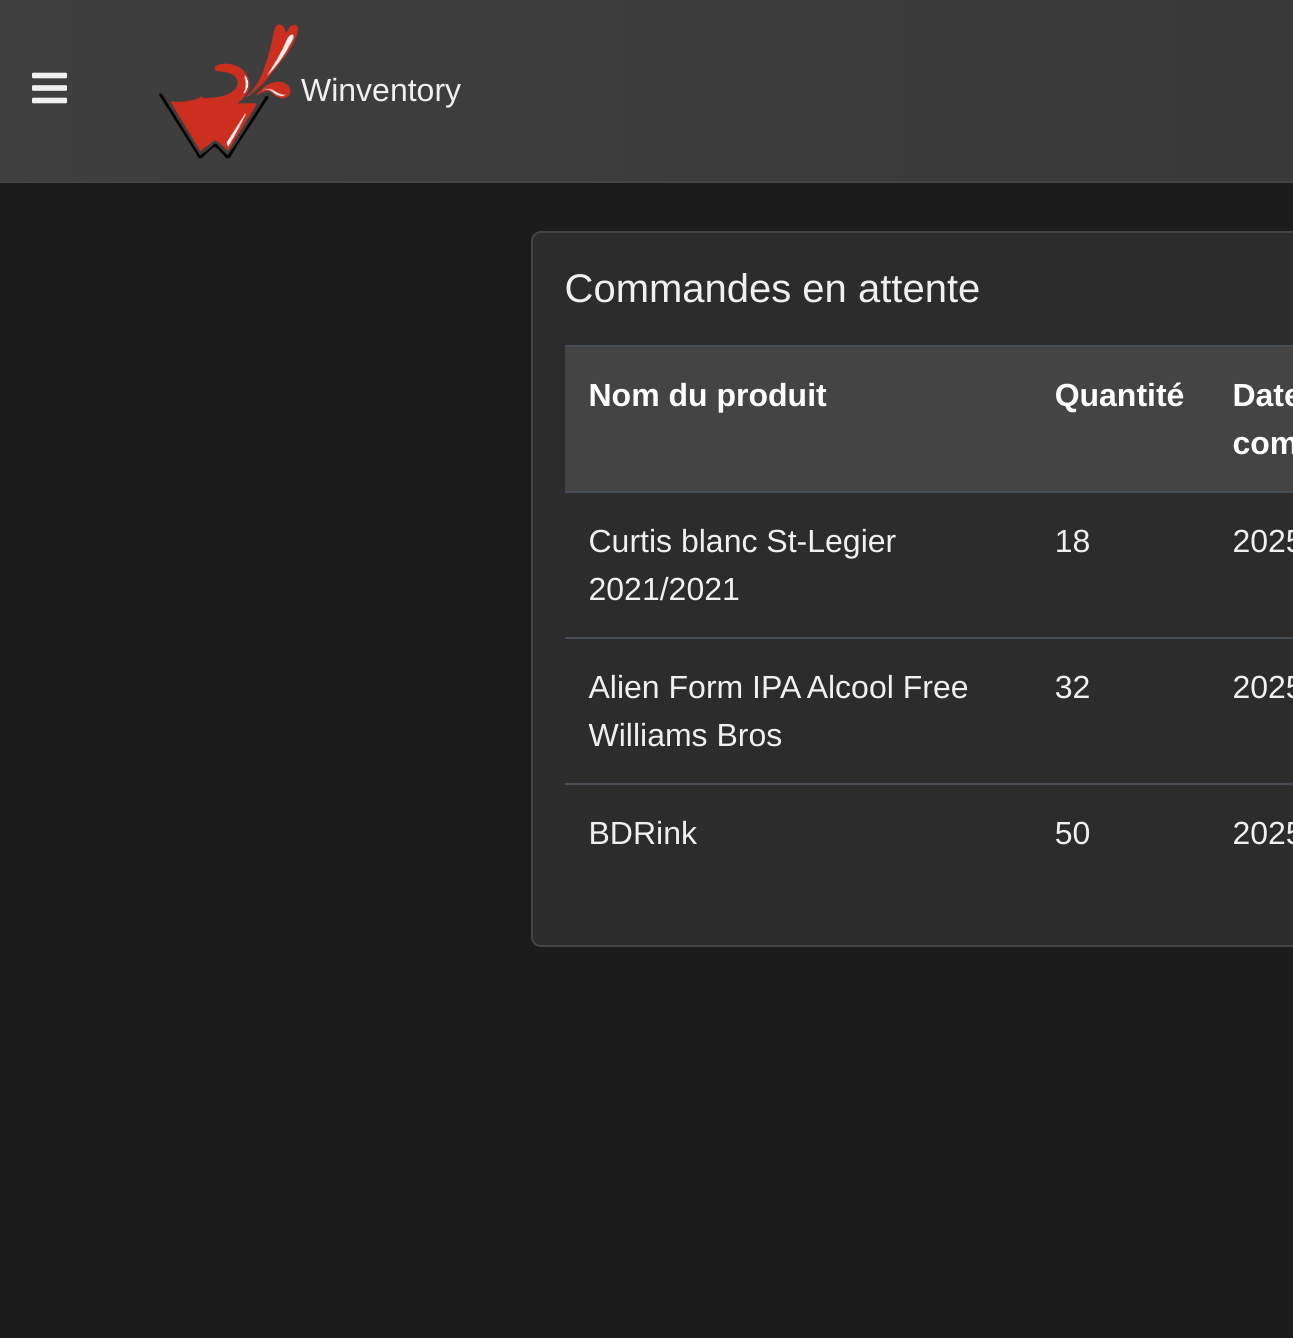
\includegraphics[width=0.7\textwidth]{images/menu}};
            % Annotation sur l'image
            \draw[green, thick] (-4.3,4.2) rectangle (-1.5,5.7);
        \end{tikzpicture}
        \caption{Utilisateur enregistré}
    \end{figure}
    \newline
    Les autres pages sont accessibles depuis le menu déroulant présent dans la barre de menu (cf. Figures 2 et 3)
    \begin{figure}[H]
        % Première image dans une minipage
        \begin{tikzpicture}
            % --- Première image ---
            \node[anchor=north west] (img1) at (0,0) {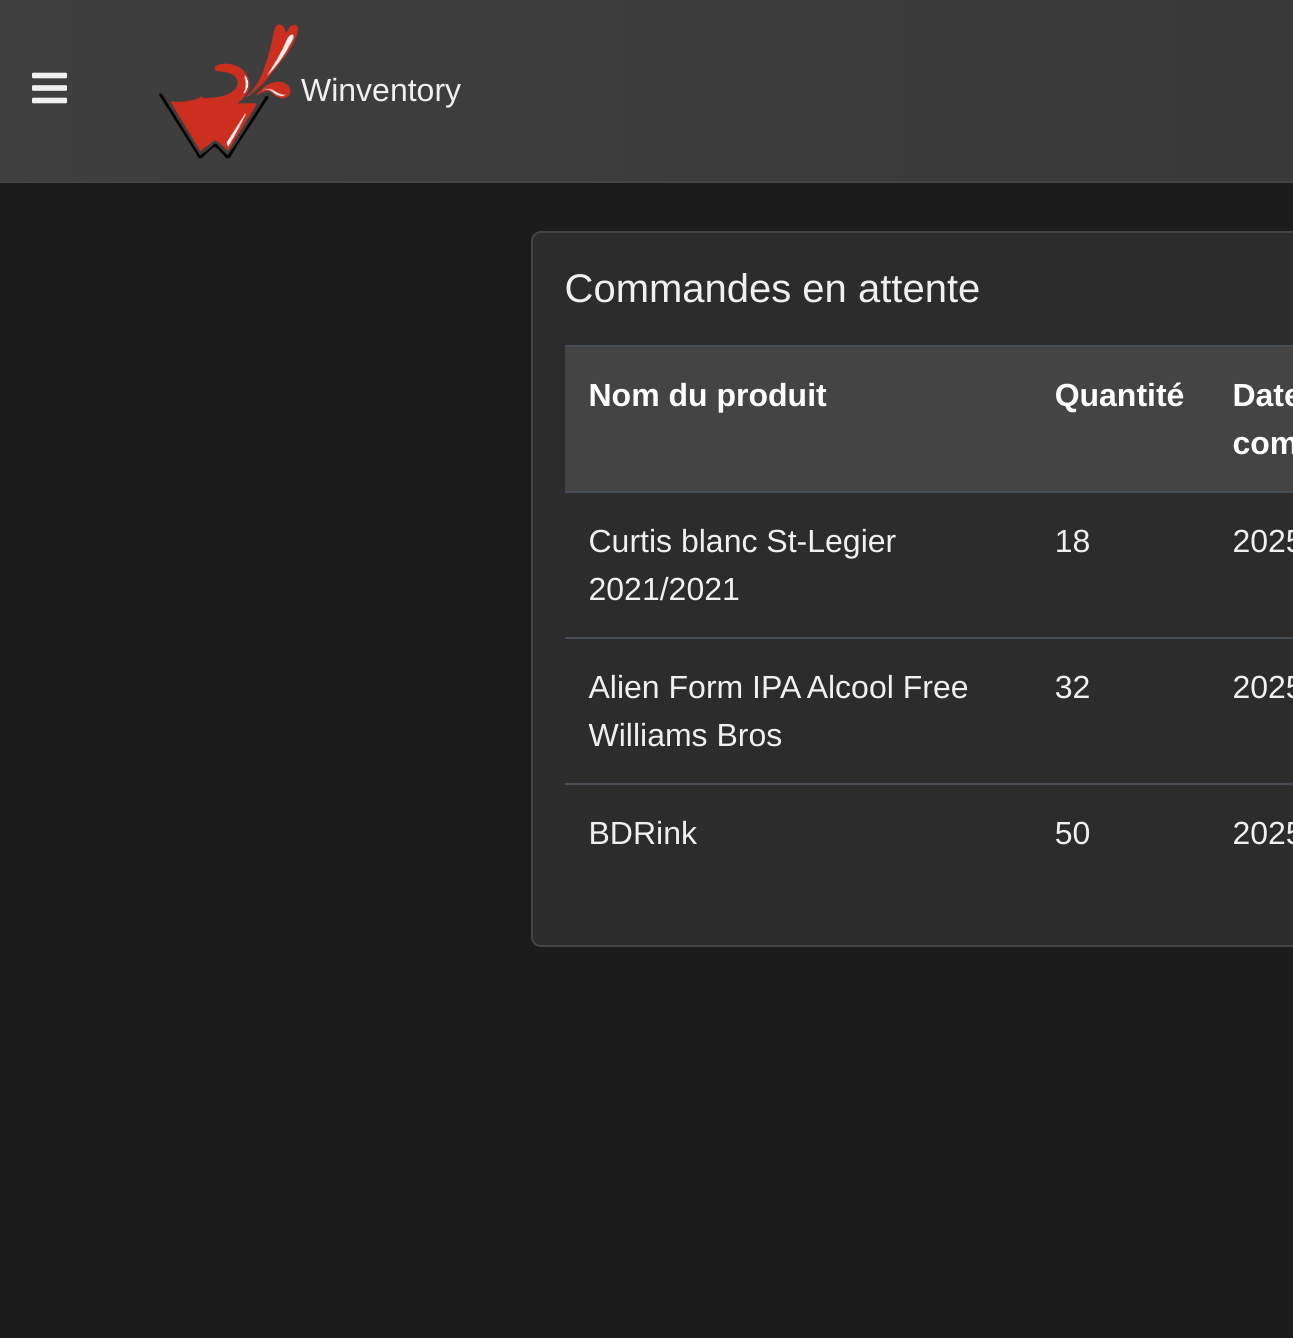
\includegraphics[width=0.45\textwidth]{images/menu}};
            % Annotation sur l'image
            \draw[green, ultra thick] (0,-1.2) rectangle (1,-0.2);
            \hspace{0.2\textwidth}
            \node[anchor=north west] (img1) at (6,0) {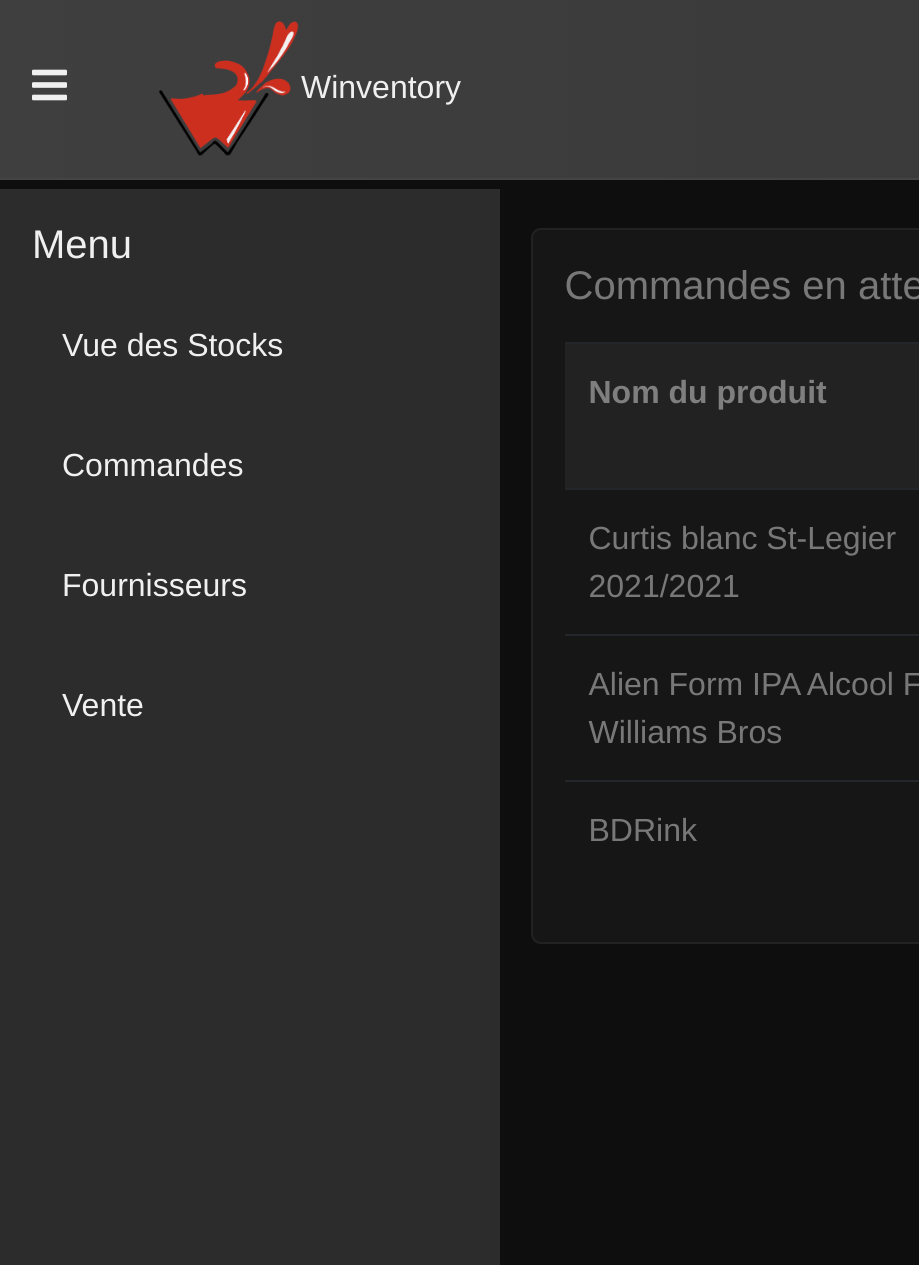
\includegraphics[width=0.45\textwidth]{images/menu_deroulant}};
            \draw[->, double, line width=4, green] (3,-4) -- (6,-4)
        \end{tikzpicture}
        \caption{Menu déroulant fermé\\ Figure 3: Menu déroulant ouvert}
    \end{figure}

    \newpage
    \subsection*{Page de connexion}
    \addcontentsline{toc}{subsection}{Page de connexion}

    La page d'accueil comporte deux champs de texte et deux boutons:
    \newline
    \begin{figure}[H]
        \begin{center}
            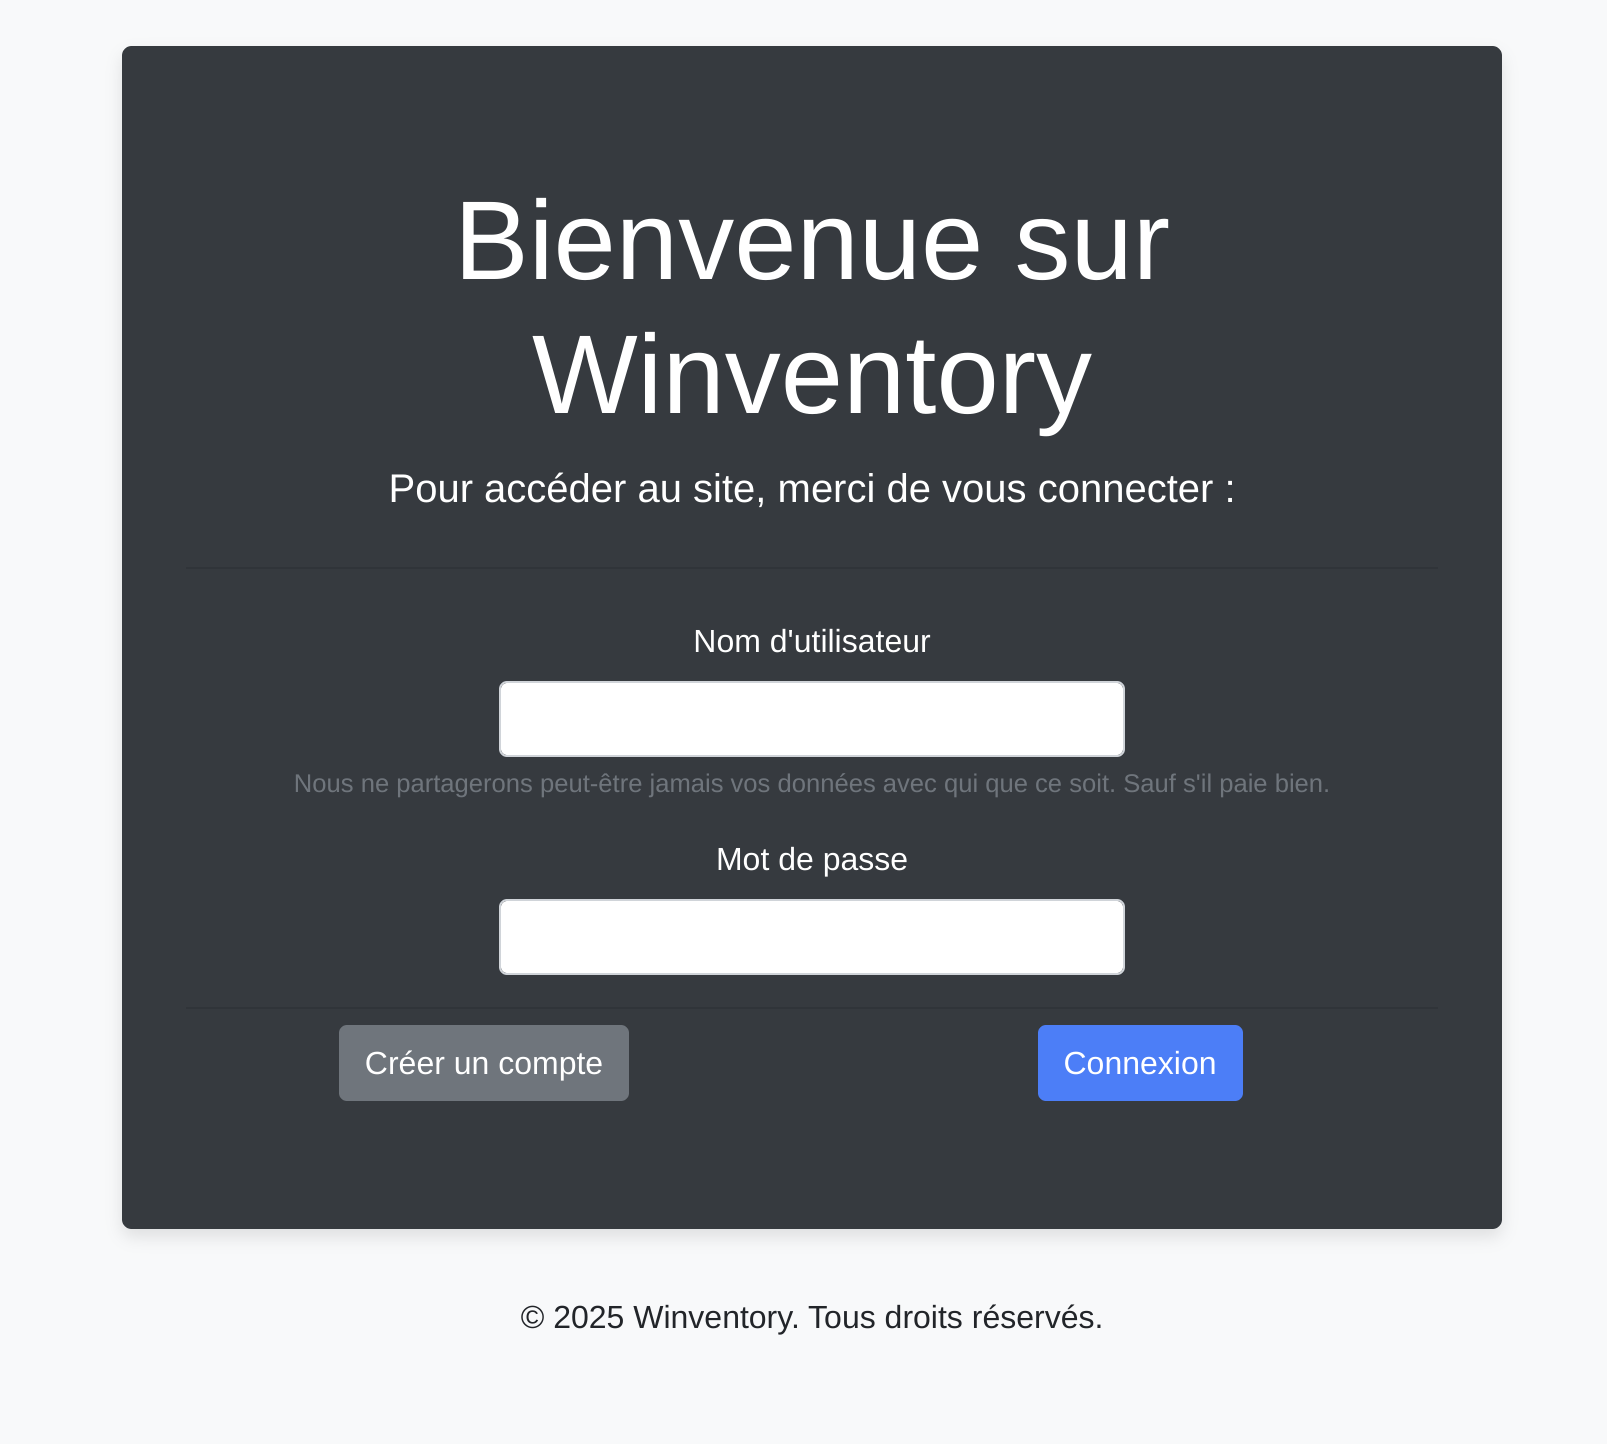
\includegraphics[scale=0.2]{images/index1}
            \caption{Page de connexion}
        \end{center}
    \end{figure}
    Si l'utilisateur a déjà un profil, il peut directement se connecter en remplissant les champs et en appuyant sur le
    bouton "Connexion". Si ce n'est pas le cas, l'utilisateur peut se créer un compte en cliquant sur le bouton "Créer un compte":
    \newline
    \newline
    Lorsque l'utilisateur clique sur le bouton "Créer un compte", il est redirigé sur la page d'enregistrement de l'utilisateur.

%    \begin{figure}[H]
%        % Première image dans une minipage
%        \begin{tikzpicture}
%            % --- Première image ---
%            \node[anchor=south west] (img1) at (0,0) {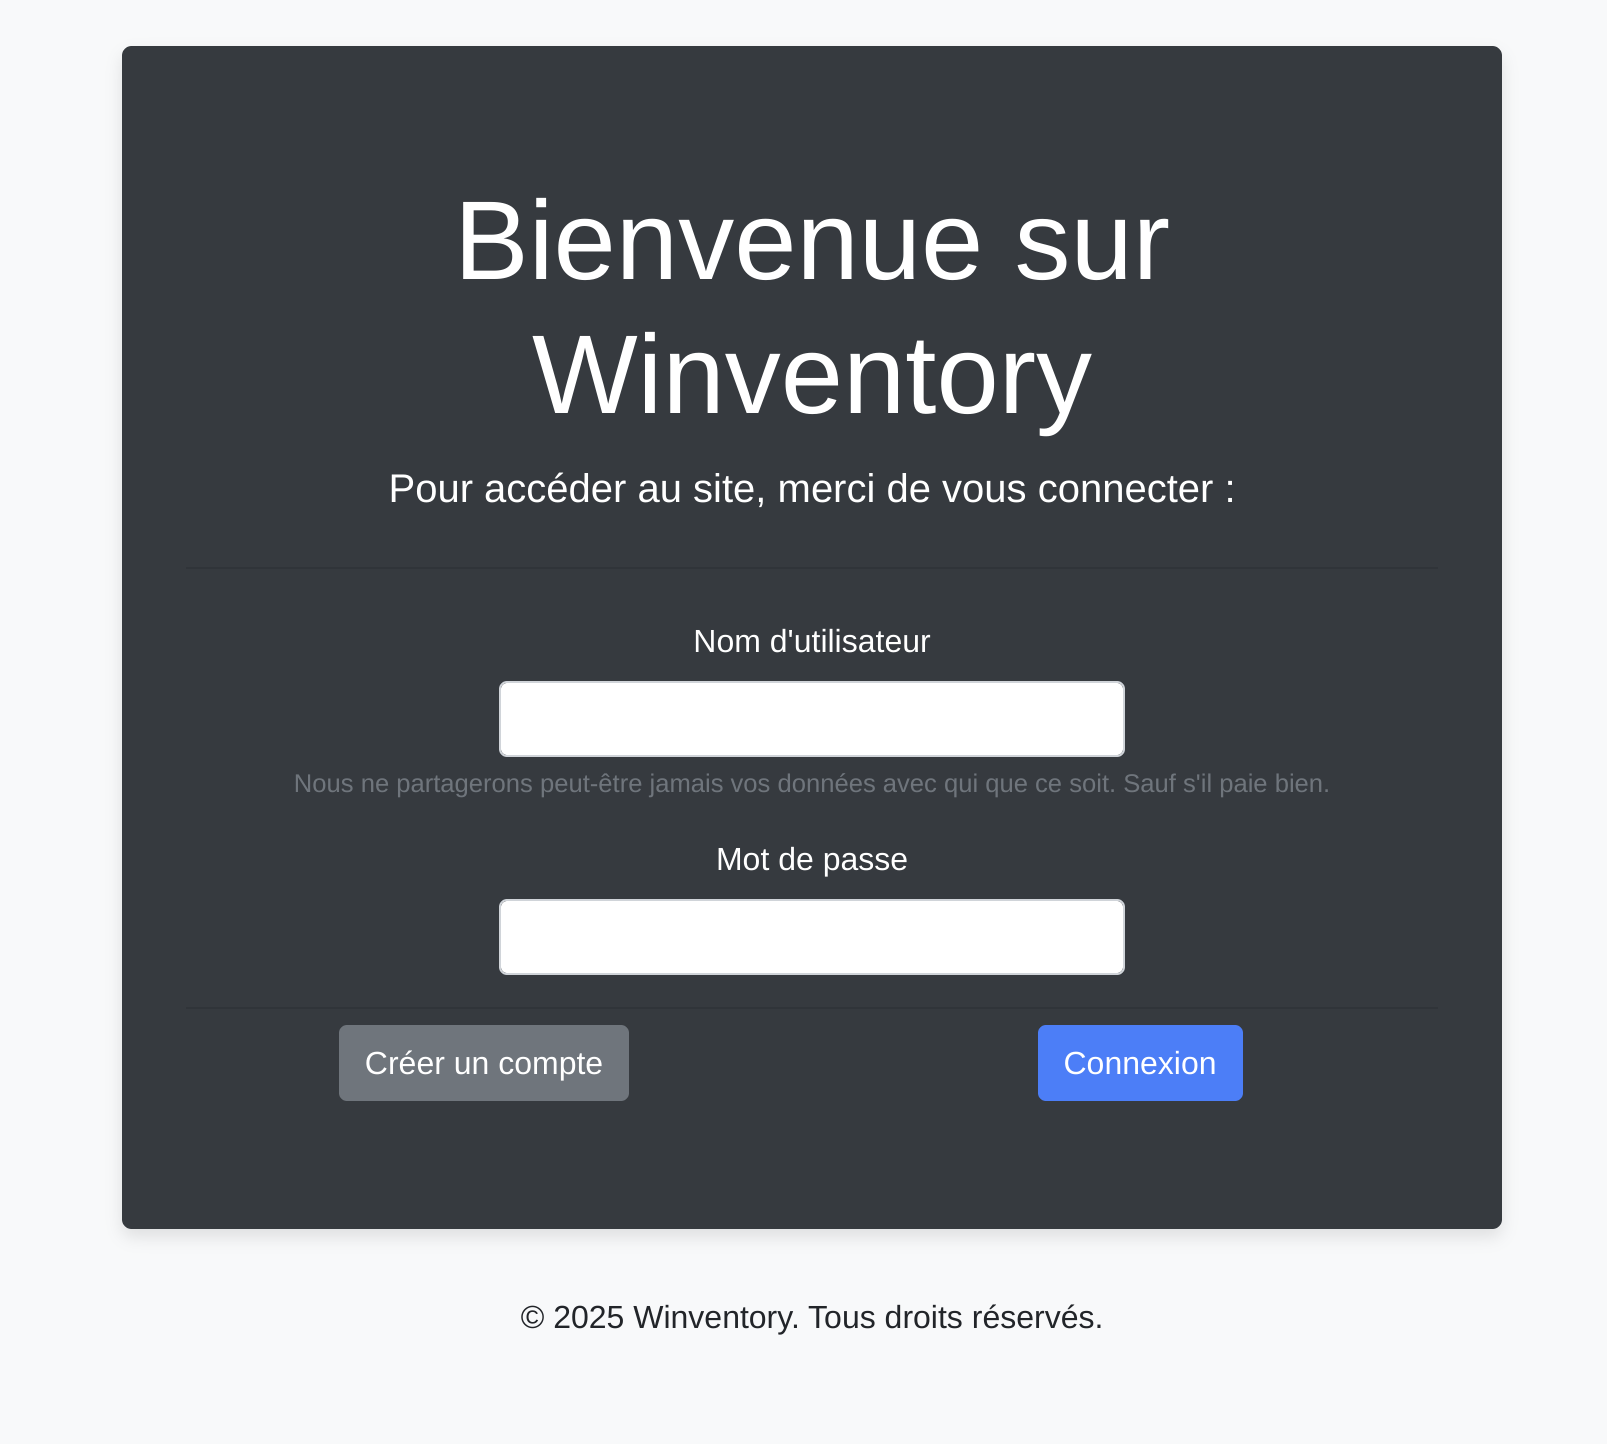
\includegraphics[width=0.5\textwidth]{images/index1}};
%            % Annotation sur la première image
%            \draw[red, thick] (1, 1) ellipse (0.5cm and 0.25cm);
%            \end{tikzpicture}
%        \caption{Cliquer pour créer un compte \\ Figure 2: Cliquer pour se connecter}
%    \end{figure}
    \newpage
    \subsection*{Page d'enregistrement}
    \addcontentsline{toc}{subsection}{Page d'enregistrement}

    Cette page permet à l'utilisateur de s'enregistrer pour avoir accès à l'application.

    \begin{figure}[H]
        \begin{center}
            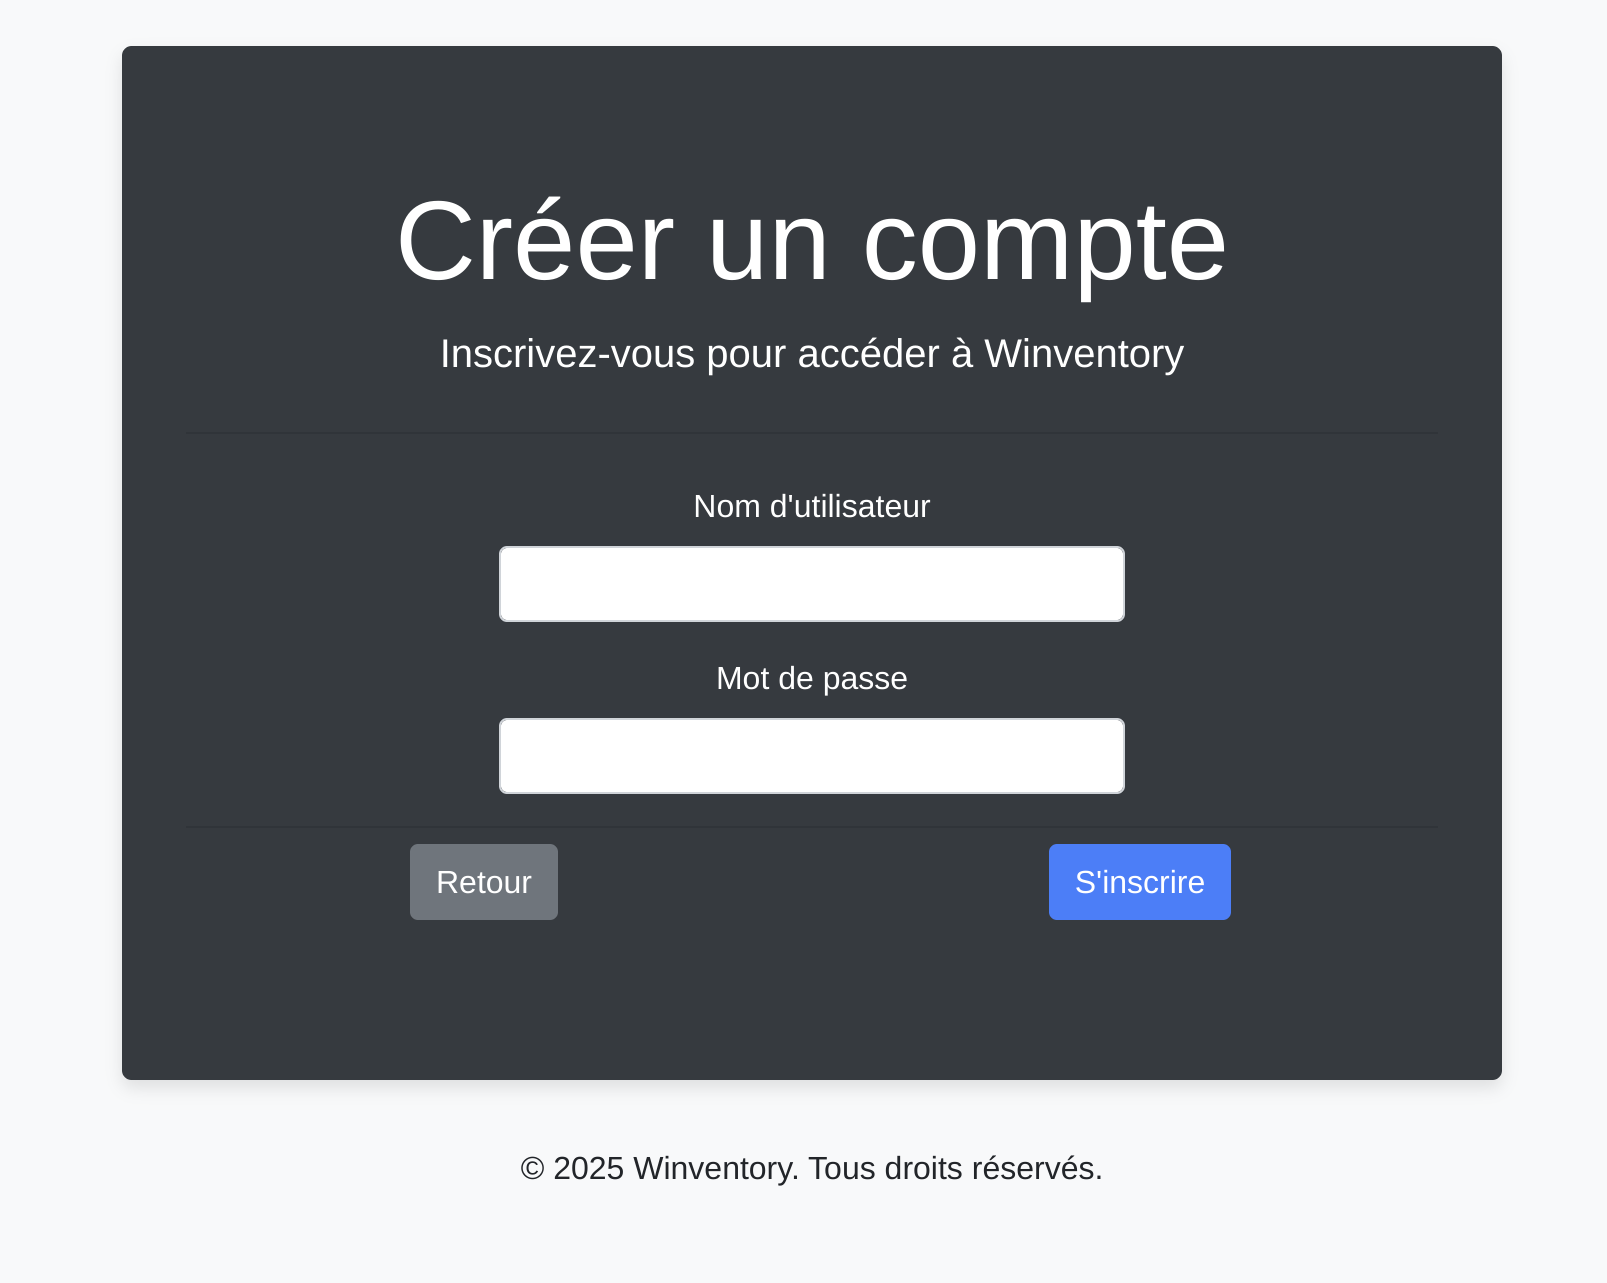
\includegraphics[scale = 0.2]{images/register}
            \caption{Page d'enregistrement}
        \end{center}
    \end{figure}
    Pour s'enregistrer, il suffit simplement de trouver un nom et un mot de passe et de cliquer sur le bouton "S'inscrire".
    Lorsque le nouvel utilisateur clique sur le bouton "S'inscrire", un label rouge s'affiche, indiquant si les informations de l'utilisateur
    sont déjà utilisées ou si l'utilisateur a été correctement enregistré.
    \begin{figure}[H]
        \centering
        \begin{tikzpicture}
            \node{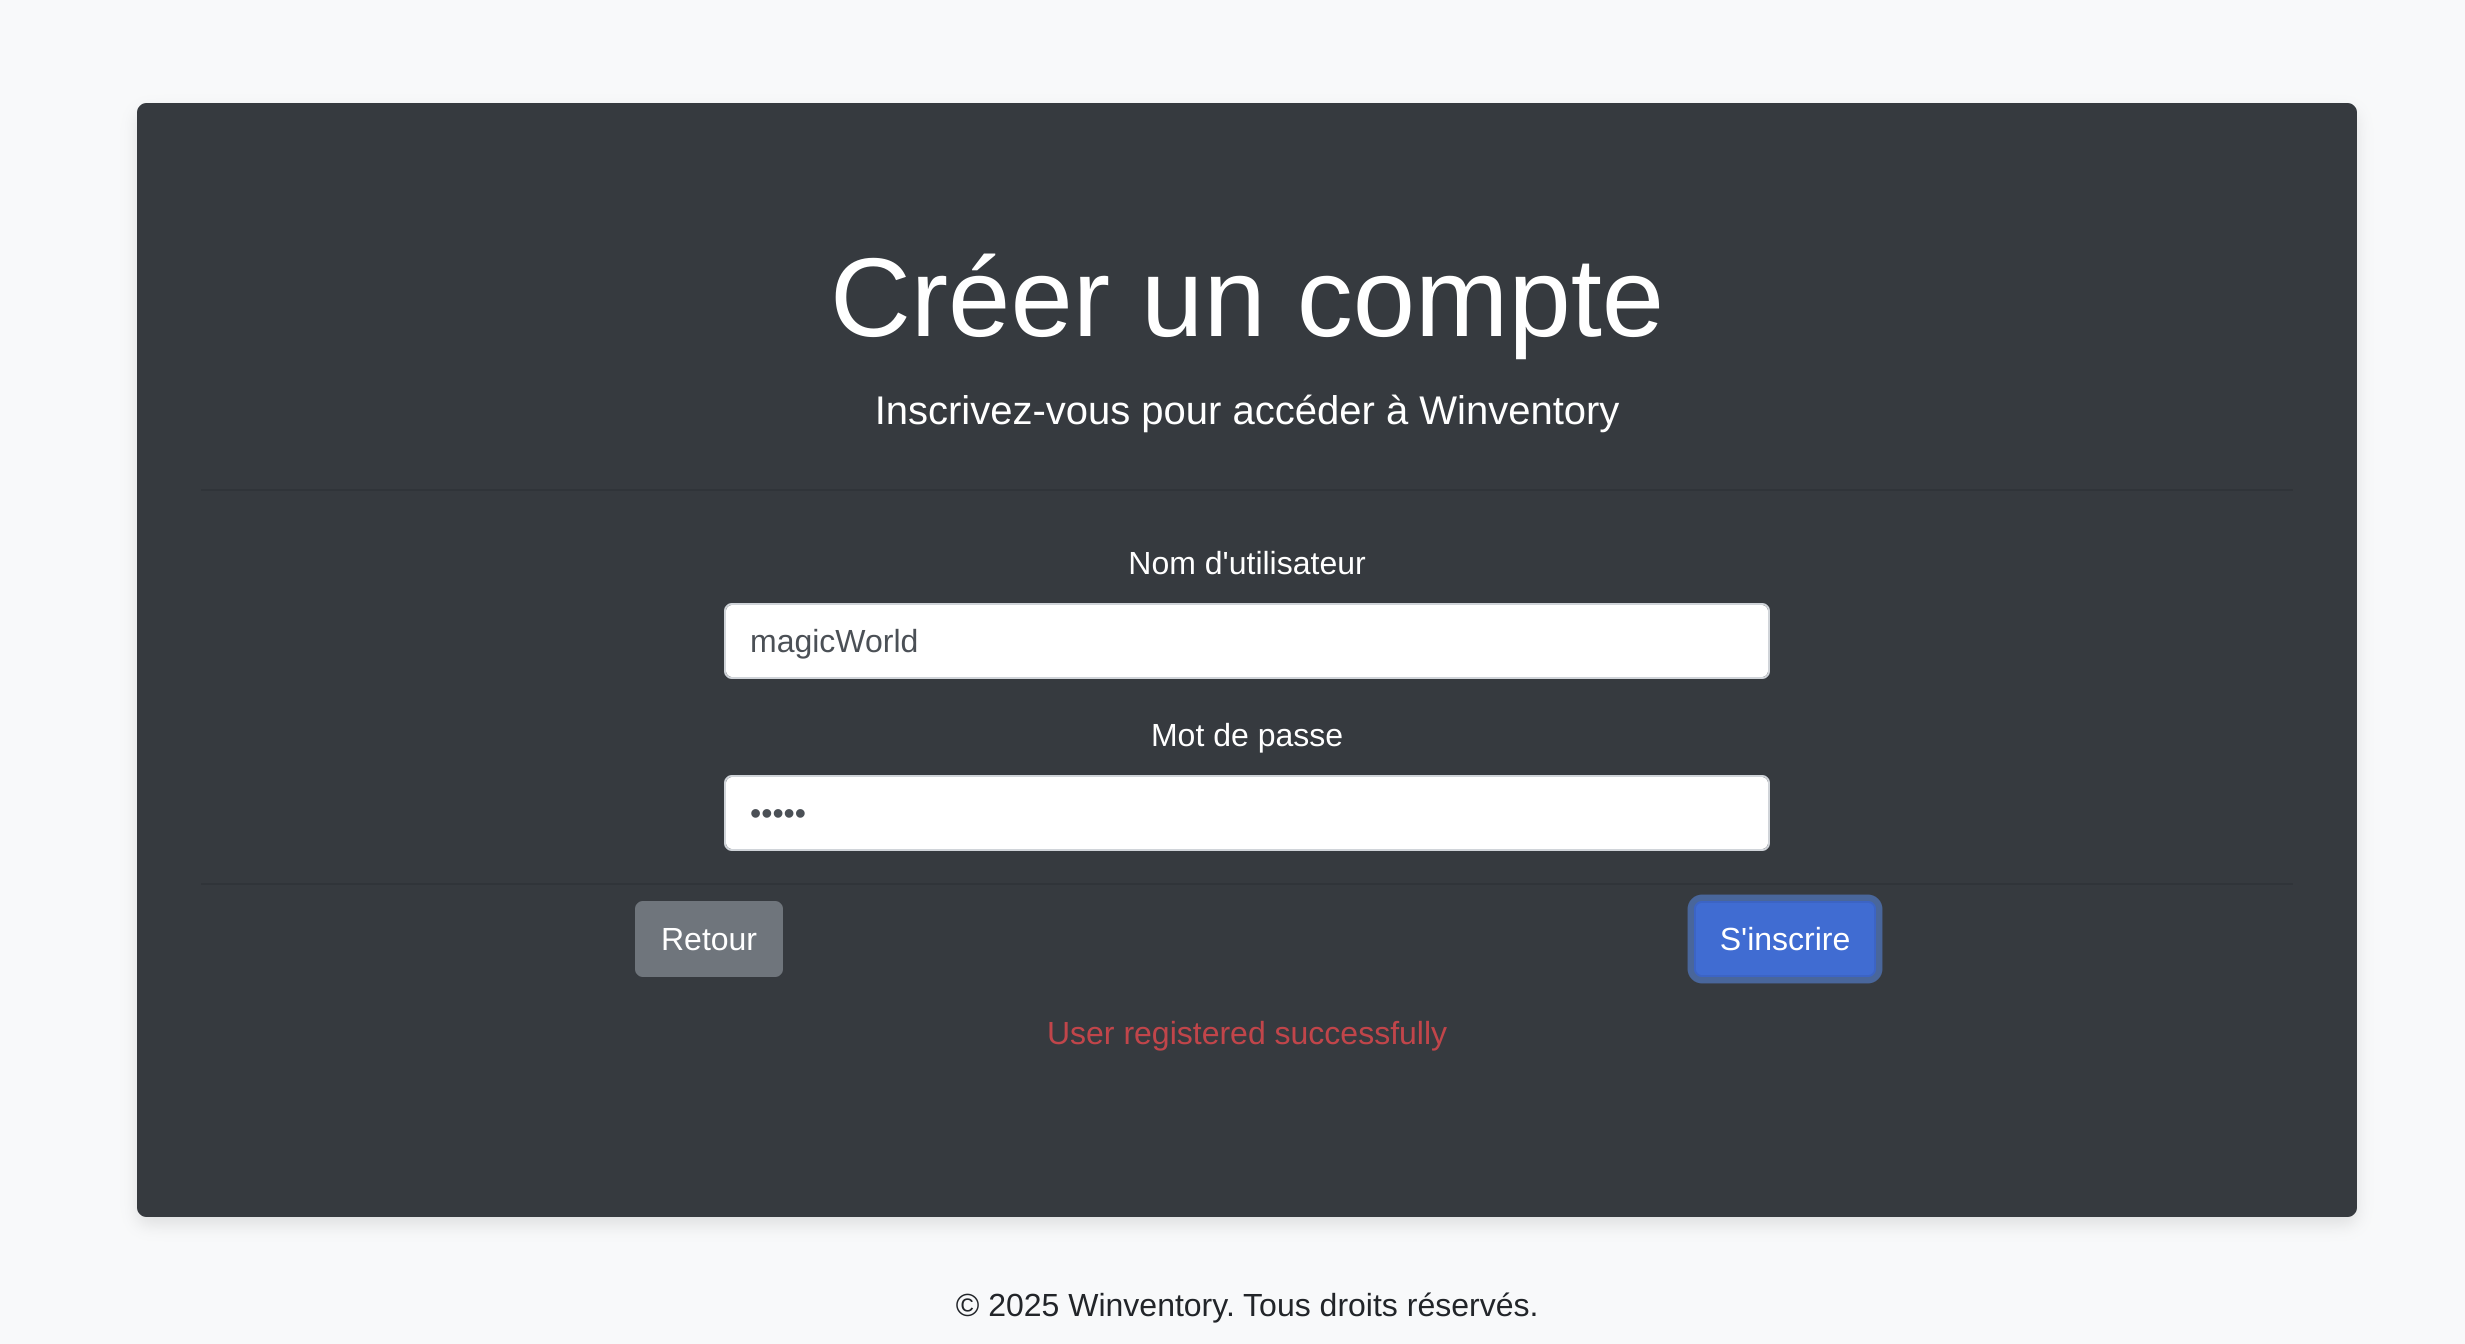
\includegraphics[width=0.7\textwidth]{images/registerDone}};
            % Annotation sur l'image
            \draw[green, thick] (-1.5,-1.9) rectangle (1.5,-1.4);
        \end{tikzpicture}
        \caption{Utilisateur enregistré}
    \end{figure}
    L'utilisateur peut alors retourner sur la page de connexion et se connecter avec le login qu'il vient de créer.

    \newpage
    \subsection*{Page d'accueil}
    \addcontentsline{toc}{subsection}{Page d'accueil}
    \begin{figure}[H]
        \begin{center}
            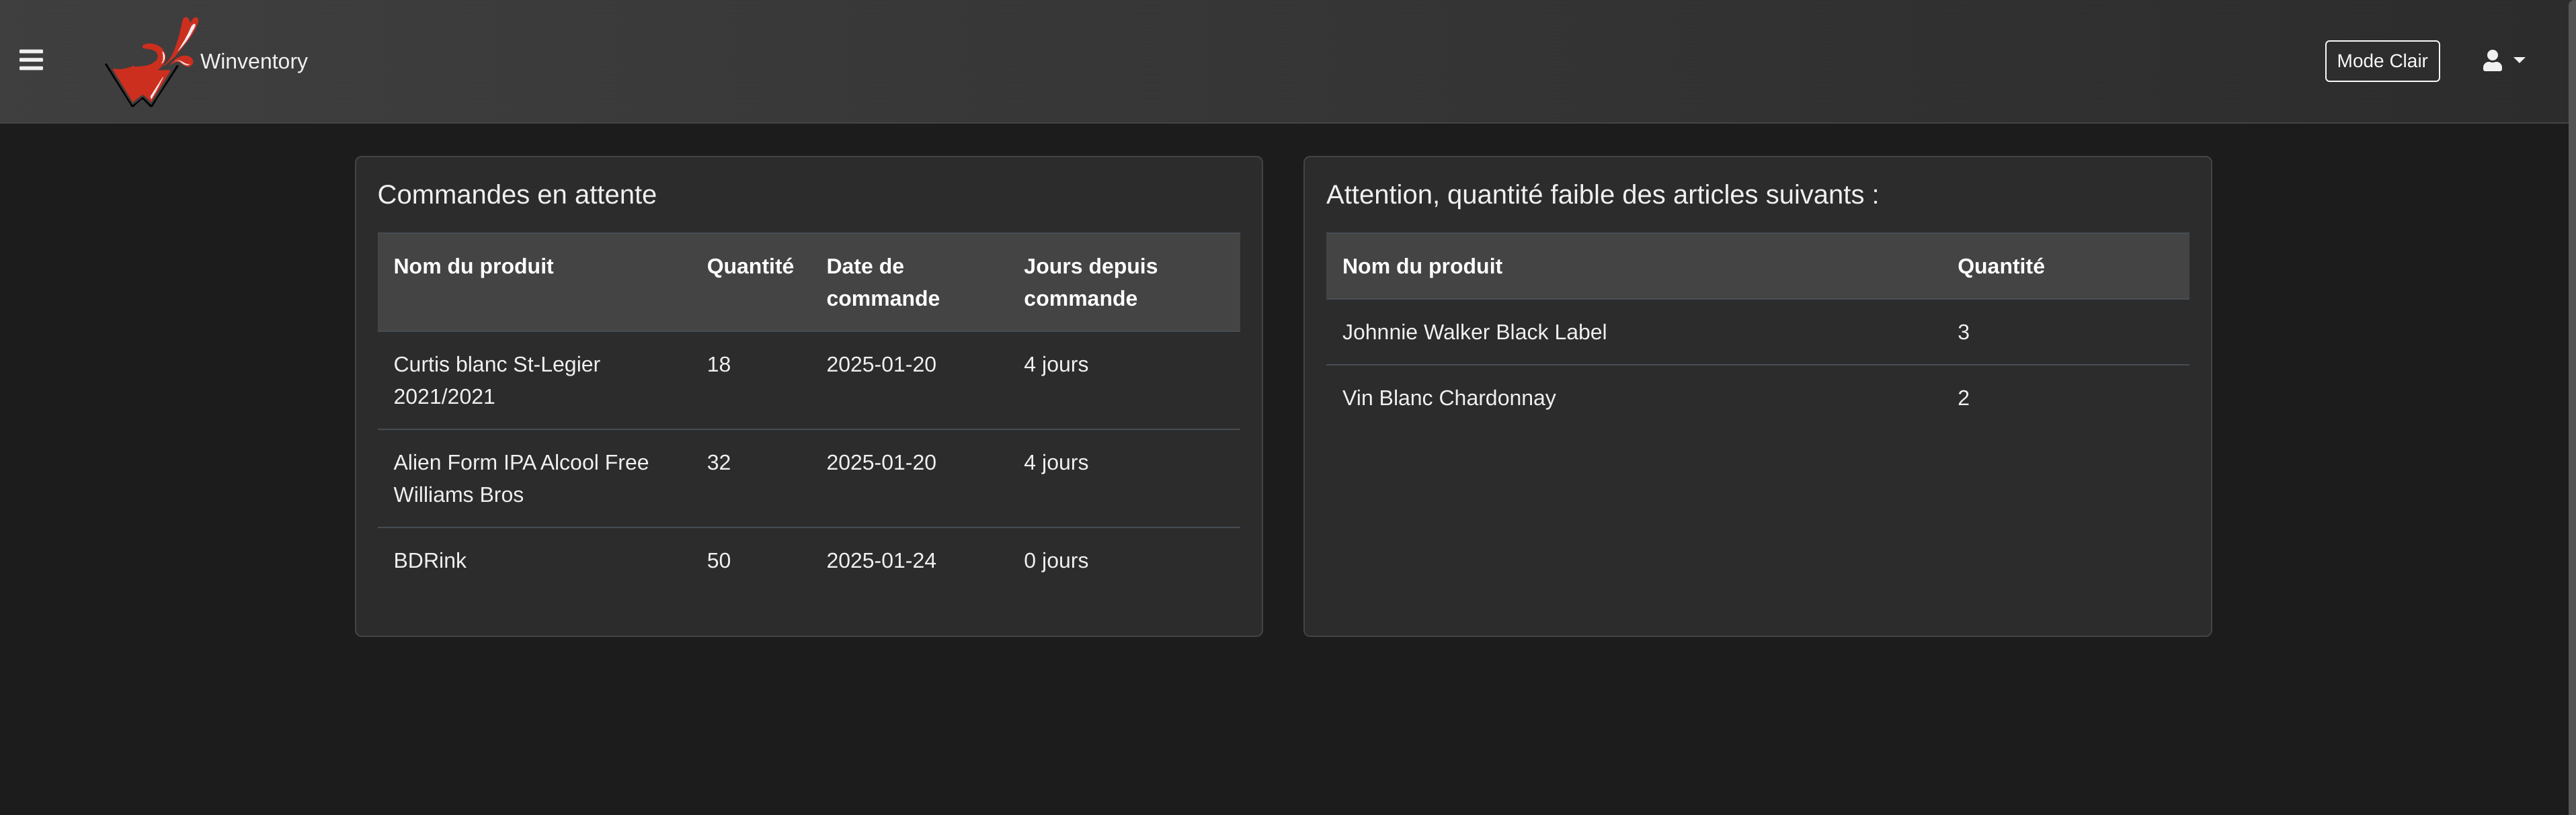
\includegraphics[width =\textwidth]{images/pageAccueil}
            \caption{Page d'accueil}
        \end{center}
    \end{figure}
    Sur cette page, on peut voir deux tableaux:
    \begin{enumerate}
        \item Les commandes en attente
        \item Les articles dont la quantité en stock est basse
    \end{enumerate}

    \subsubsection*{Commandes en attente}
    \addcontentsline{toc}{subsubsection}{Commandes en attente}
    Ce tableau permet de percevoir toutes les commandes qui ont été passées mais qui ne sont pas encore "arrivées", elles sont
    donc en attente et il faut les valider pour que leurs valeurs soient enregistrées et appliquées dans la vue des stocks.
    \newline
    \newline
    Pour les approuver, il suffit de cliquer sur l'article dont il est question et la fenêtre suivante s'affiche:
    \begin{figure}[H]
        \begin{center}
            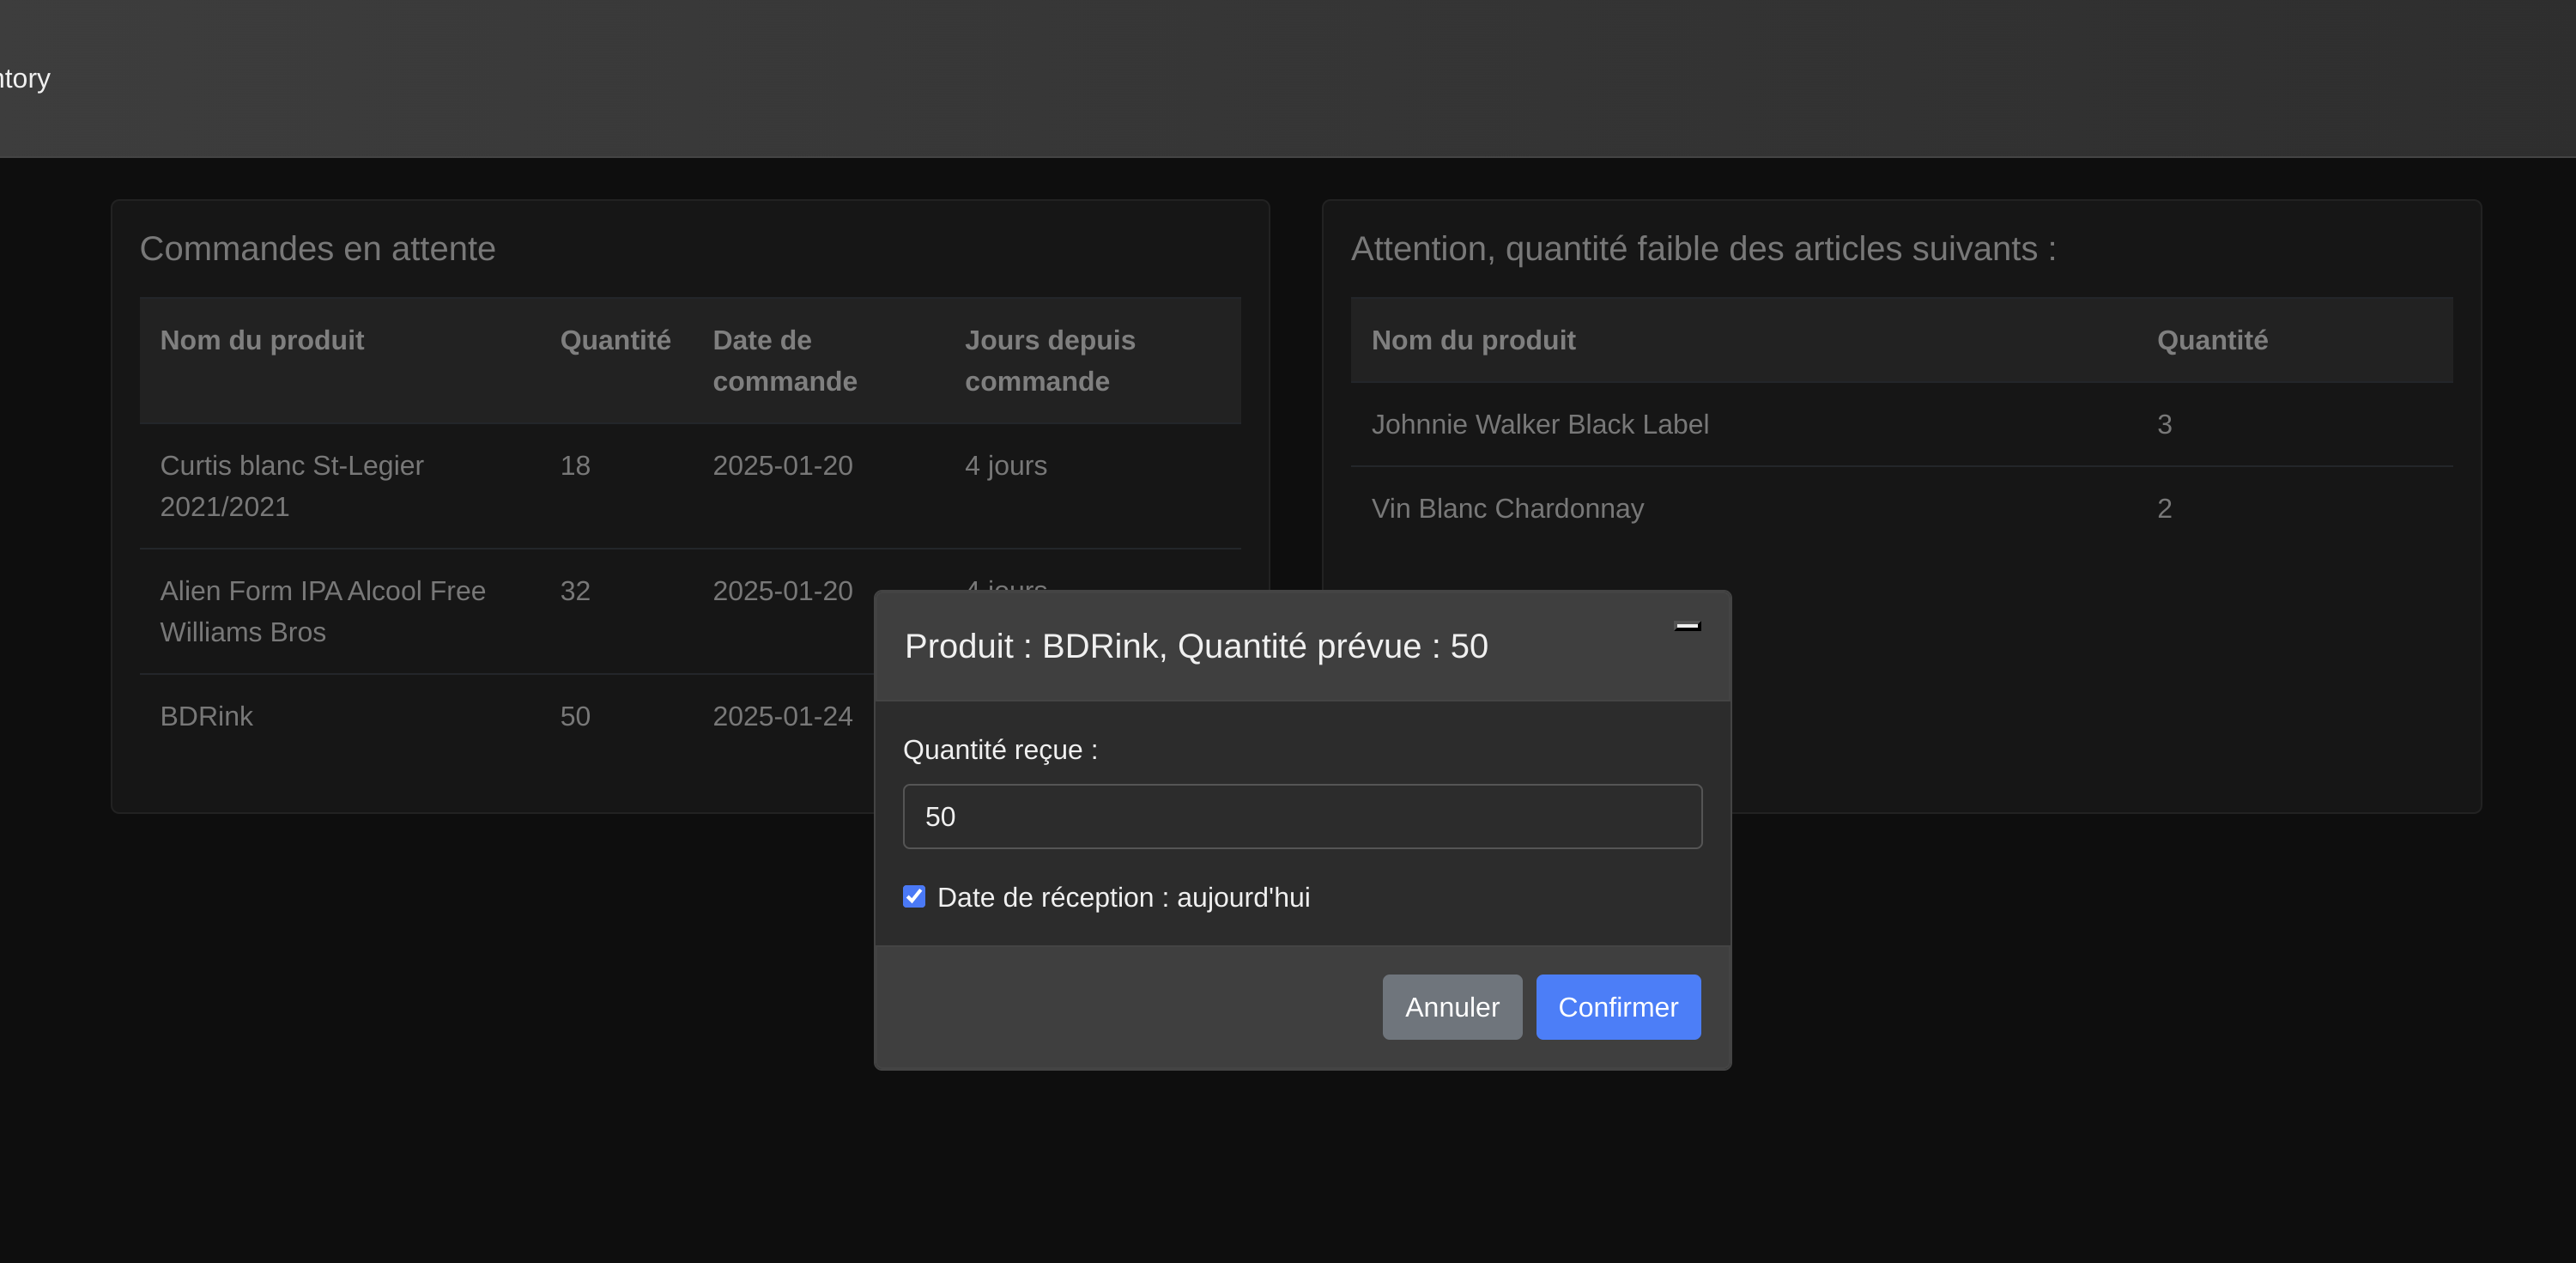
\includegraphics[width = 0.8\textwidth]{images/commandeEnAttente}
            \caption{Approuver la commande}
        \end{center}
    \end{figure}
    On peut alors modifier la quantité reçue si cette dernière ne correspond pas à la livraison réelle et modifier la date
    de réception (si jamais la modification des stocks est faite en retard).
    \newline
    Lorsque la commande est enregistrée, elle disparait du tableau "Commandes en attente".

    \subsubsection*{Articles dont les stocks sont bas}
    \addcontentsline{toc}{subsubsection}{Articles dont les stocks sont bas}
    Ce tableau affiche simplement les articles dont la quantité est faible. Cela permet de passer commande auprès
    des fournisseurs avant d'être en rupture de stock.


    \subsection*{Vue des stocks}
    \addcontentsline{toc}{subsection}{Vue des stocks}

    \newpage
    \subsection*{Formulaire de commandes}
    \addcontentsline{toc}{subsection}{Formulaire de commandes}
    %%TODO

    \newpage
    \subsection*{Formulaire de ventes}
    \addcontentsline{toc}{subsection}{Formulaire de ventes}
    %%TODO

    \newpage
    \subsection*{Fournisseurs}
    \addcontentsline{toc}{subsection}{Fournisseurs}
    %%TODO

    \newpage
    \subsection*{Ajouter un fournisseur}
    \addcontentsline{toc}{subsection}{Ajouter un fournisseur}
    %%TODO

    \newpage
    \subsection*{Profil du vendeur}
    \addcontentsline{toc}{subsection}{Profil du vendeur}
    %%TODO


%%%%%%%%%%%%%%%%%%%%
%%   Bugs connus  %%
%%%%%%%%%%%%%%%%%%%%
    \section*{Bugs connus}
    \addcontentsline{toc}{section}{Bugs connus}

    \begin{itemize}
        \item Une vente peut être effectuée par un vendeur quelconque, avec un email quelconque ou pour un produit quelconque.
    \end{itemize}


%%%%%%%%%%%%%%%%%%%%
%%   Conclusion   %%
%%%%%%%%%%%%%%%%%%%%
    \section*{Conclusion}
    \addcontentsline{toc}{section}{Conclusion}

%%%%%%%%%%%%%%%%%%%%
%%     Annexes    %%
%%%%%%%%%%%%%%%%%%%%
    \appendix
    \appendixpage
    \addappheadtotoc
    \section{Annexe 1 - Accès à l'application, DAI}
    (page suivante)
    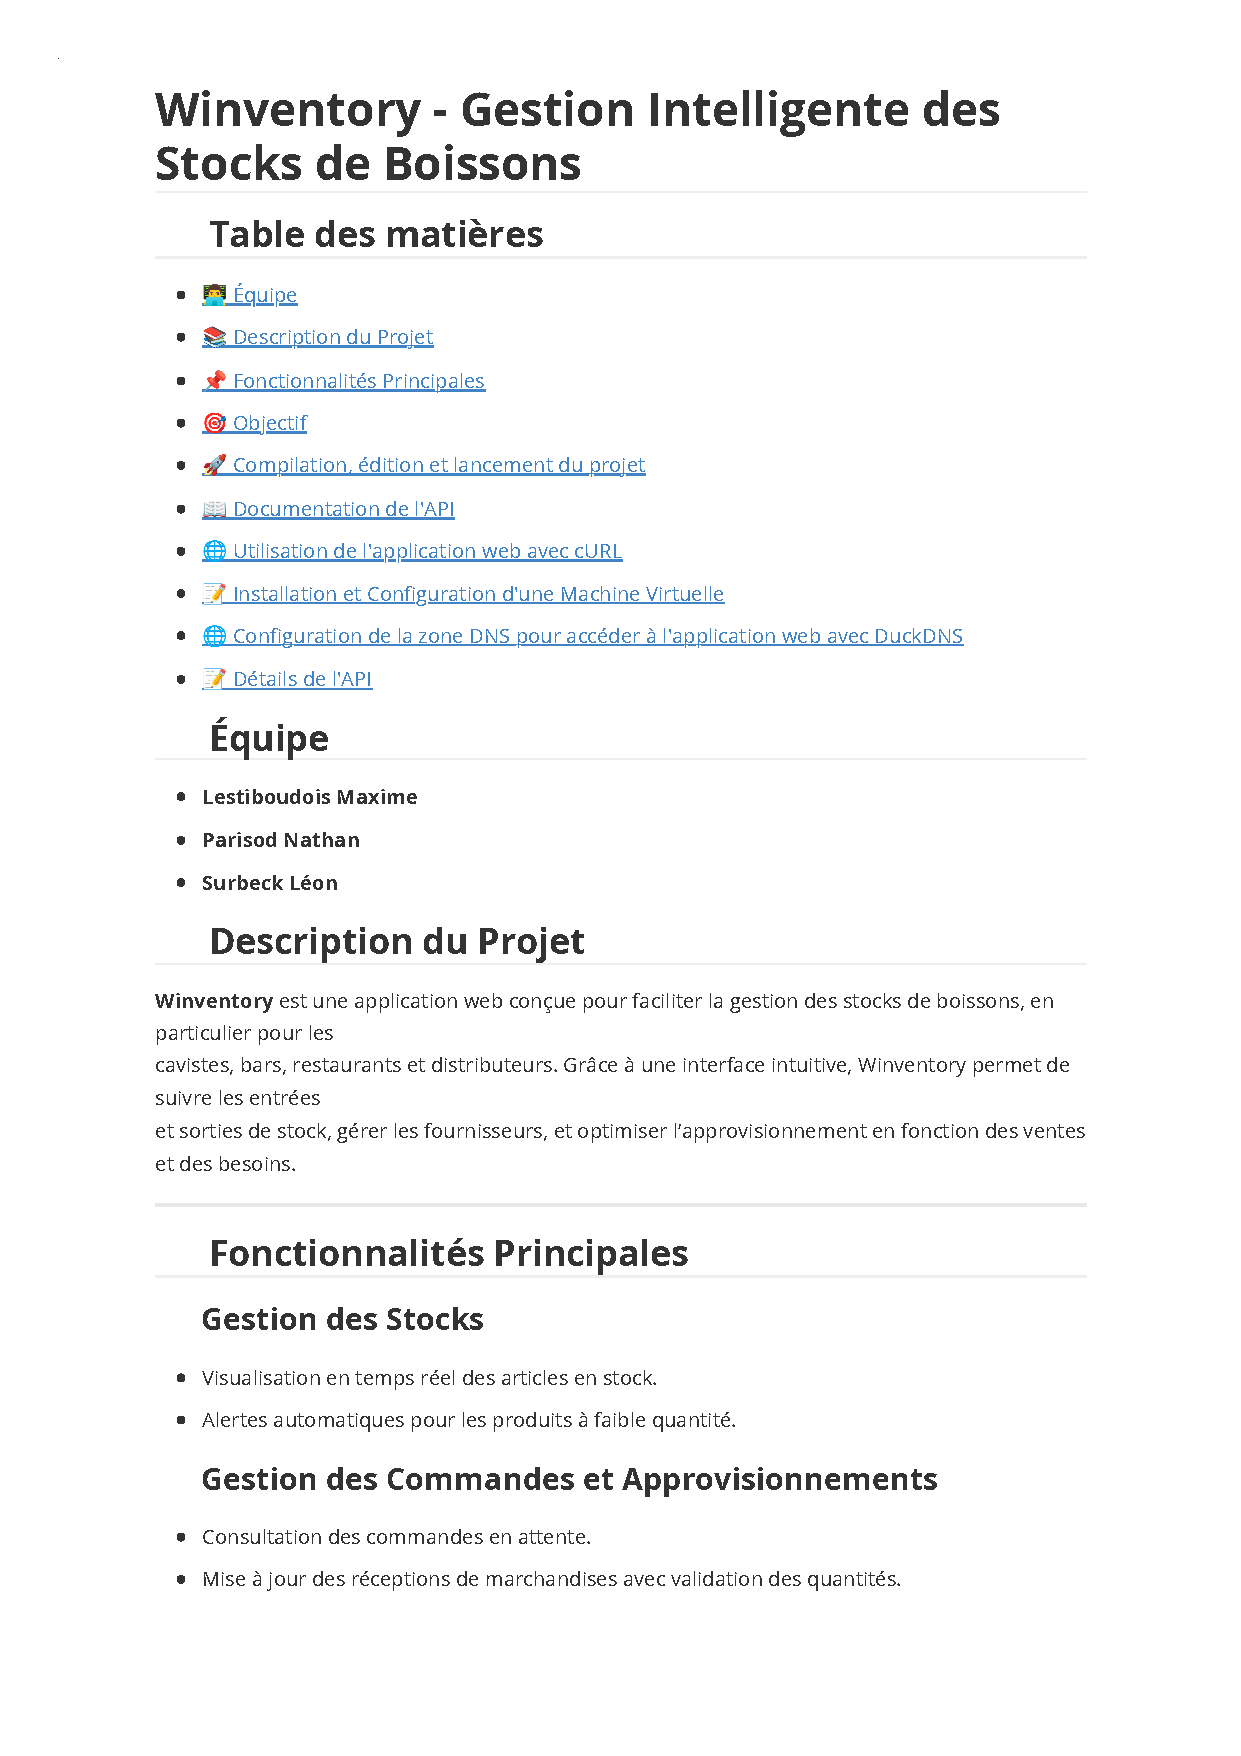
\includepdf[pages=-, pagecommand = {\thispagestyle{plain}}]{oldReadme.pdf}

\end{document}